% =============================================================================
% FAECO 中文期刊版式（计算机辅助设计与图形学学报模板近似）
% 字体说明：模板要求方正书宋_GBK/方正仿宋_GBK/黑体/Times New Roman。
% 方正 GBK 字库为商业字体，需作者自行购买安装；当前以系统宋体/黑体/仿宋近似。
% 安装方正字库后，将下方 FZ 字体变量替换为对应方正字体名即可。
% =============================================================================
\documentclass[twocolumn,10pt,fontset=windows]{ctexart}

% -----------------------------------------------------------------------------
% 字体（方正 GBK 安装后替换此处）
%   正文:    \setCJKmainfont{方正书宋_GBK}
%   标题:    \setCJKsansfont{方正黑体_GBK}
%   仿宋:    \setCJKfamilyfont{fzfs}{方正仿宋_GBK}
% 当前用系统字体近似（fontset=windows: 宋体/黑体/楷体/仿宋）
% -----------------------------------------------------------------------------
\setmainfont[Path=./fonts/,Extension=.ttf,UprightFont=times,BoldFont=timesbd,ItalicFont=timesi,BoldItalicFont=timesbi]{Times New Roman}
\setCJKmainfont[Path=./fonts/,Extension=.ttf]{FZShuSong-Z01}
\setCJKsansfont[Path=./fonts/,Extension=.ttf]{SimHei}
\newCJKfontfamily\songfamily[Path=./fonts/,Extension=.ttf]{FZShuSong-Z01}
\newCJKfontfamily\fangfamily[Path=./fonts/,Extension=.ttf]{FZFangSong-Z02}
\newCJKfontfamily\heifamily[Path=./fonts/,Extension=.ttf]{SimHei}
\usepackage{amsmath,amssymb}
\usepackage{newtxmath}
\let\songti\songfamily\let\heiti\heifamily\let\fangsong\fangfamily
\usepackage{booktabs}
\usepackage{graphicx}
\usepackage{subfig}
\usepackage{float}
\usepackage{array}
\usepackage[nocompress]{cite}
\usepackage[hidelinks]{hyperref}
\usepackage{xurl}
\usepackage{algorithm}
\usepackage{algpseudocode}
\usepackage{multirow}
\usepackage{geometry}
\usepackage{placeins}
% 注意：双栏模式下  遇到待排浮动体会退化为 \clearpage，造成栏底留白、
% 正文后移、参考文献被挤成孤儿末页。本稿正文已不再插入 （正文仅保留
% 图 2 之后一处用于约束全宽浮动体）；压页请优先调整浮动体参数，勿缩字体/行距/砍内容。
\usepackage{dblfloatfix}
\usepackage[noshrink,nospread]{flushend}

% 版面：A4 双栏，栏宽 21.59 字符、栏间距 3 字符（以 3zw 近似）
\geometry{a4paper,left=2.0cm,right=2.0cm,top=2.1cm,bottom=2.1cm,columnsep=31.5pt}

\renewcommand{\eqref}[1]{\textup{（\ref{#1}）}}
\graphicspath{{../figures/}}
\setlength{\emergencystretch}{3em}
\Urlmuskip=0mu plus 3mu\relax
\raggedbottom
\setlength{\floatsep}{6pt plus 2pt minus 2pt}
\setlength{\textfloatsep}{8pt plus 2pt minus 2pt}
\setlength{\intextsep}{6pt plus 2pt minus 2pt}
\setlength{\dblfloatsep}{6pt plus 2pt minus 2pt}
\setlength{\dbltextfloatsep}{8pt plus 2pt minus 2pt}

% -----------------------------------------------------------------------------
% 标题层级（模板：1级11.5pt黑体 / 2级五号黑体 / 3级10pt书宋）
% -----------------------------------------------------------------------------
\ctexset{
  section = {format=\heiti\fontsize{11.5}{15}\selectfont, beforeskip=6pt, afterskip=4pt},
  subsection = {format=\heiti\fontsize{10.5}{14}\selectfont, beforeskip=5pt, afterskip=3pt},
  subsubsection = {format=\songti\fontsize{10}{13}\selectfont, beforeskip=4pt, afterskip=2pt}
}

% 图题（书宋9pt）、表题（黑体9pt）、表注/分图题（书宋8pt）
\usepackage{caption}
\DeclareCaptionFont{songti}{\songti}
\DeclareCaptionFont{heiti}{\heiti}
\captionsetup[figure]{font={songti,small},labelfont={bf},skip=3pt}
\captionsetup[table]{font={heiti,small},labelfont={bf},skip=3pt}
% subfig is not used in this manuscript; do not configure an unused subfloat caption.
\captionsetup{labelsep=space}


\begin{document}
\pagestyle{plain}
\renewcommand{\thesection}{S\arabic{section}}
\renewcommand{\thefigure}{S\arabic{figure}}
\renewcommand{\thetable}{S\arabic{table}}
\renewcommand{\theequation}{S\arabic{equation}}
\twocolumn[
\begin{center}
{\heiti\Large FAECO：补充材料}\par
\vspace{4pt}
{\songti 主文方法细节、附加实验与验证条件}\par
\end{center}
参考文献编号沿用主文。主文的72次受控运行与以下单轮、跨测试集、策略、反馈、结构和物理实验分别保留配置，不跨族归因。原始代码、输入与测量索引见S6。
]
\section{候选构造细节}
\subsection{方法总览}\label{sec:overview}

FAECO 包含映射准备、候选生成和时序验证三个阶段，如主文图1所示。候选策略为 R、G、B 和 JOINT。

\begin{enumerate}
  \item[(a)] \textbf{映射准备}：经 Yosys 两步流程生成 SKY130 HD 映射网表 $G'$；Liberty 文件提供单元逻辑和时序信息\footnote{\url{https://github.com/google/skywater-pdk}}，BLIF 归一化与 ABC \texttt{cec}\textsuperscript{[11]} 用于组合网表回验。
  \item[(b)] \textbf{边界构造与候选实例化}：在当前违例扇入锥上求一个加权节点割，并由 STA 报告中的关键实例构造覆盖区域。覆盖优先配置先调度覆盖区域，再调度加权割区域；相同区域合并来源。区域内按实例和动作顺序枚举 R/G/B/JOINT。Liberty 函数匹配决定 R 的可用性，没有 R 候选的门仍可进入割及 G/B 枚举。OpenSTA 结果用于接受，F1--F6 用于诊断及可选反馈。
  \item[(c)] \textbf{验证与接受}：候选经库函数和结构规则筛选后，由 OpenSTA 在理想线网模式下测量 WNS/TNS；启用物理门控时，仅理想线网增益超过 10\,ps 的候选进入简化 SPEF 复测。$0<\Delta\mathrm{WNS}\le10\,$ps 的候选被阈值直接过滤，不计入 F1--F6 失效反馈；仅当候选满足式~\eqref{eq:accept} 但 SPEF 复测下 WNS 不改善时记为 F6。
\end{enumerate}

总框架见主文图1；本补充保留完整参数、枚举与失效分析。

\begin{algorithm}[H]
\footnotesize
\caption{FAECO 修复流程示意}\label{alg:main}
\begin{algorithmic}[1]
\Require 映射网表 $G'$、时序约束 $T$、工艺库 $\mathcal{L}$
\Ensure 修复后网表 $G^*$、接受候选集合 $\mathcal{A}$
\State 保存基线网表 $G_0\gets G'$，初始化当前网表 $N\gets G_0$、$G^*\gets G_0$、$\mathcal{A}\gets\emptyset$ 和搜索权重 $\lambda$
\Repeat
  \State 从当前网表$N$的固定目标端点$t$提取扇入锥，必要时按深度分治
  \State 按算法~\ref{alg:regions}构造、合并并调度区域，实例化 R/G/B/JOINT 动作
  \State 对候选执行局部功能/结构检查和 OpenSTA 测量
  \State 对满足物理门控条件的候选进行简化 SPEF 复测
  \State 若候选满足式~\eqref{eq:accept} 并在启用物理门控时通过简化 SPEF 复测，则将其加入 $\mathcal{A}$，并将该候选应用于当前网表、提交为下一轮评估基准（$N\gets N+\Delta$），同时更新最优网表 $G^*$。同一轮内多个候选共享同一基准 $N$ 且互不叠加；该轮一旦提交，基于旧基准的其余候选即作废，提交后更新报告序列$P$，在原目标端点$t$重提扇入锥并重新生成候选
  \State \textbf{若启用失效反馈控制}，触发 F1--F6 的失效候选按对应失效类型记录，并更新后续搜索分析的输入；固定权重配置仅记录失效类型、不更新权重。因 10\,ps 阈值直接过滤的候选不参与失效反馈
\Until{无时序违例、候选耗尽或达到停止条件}
\State \Return $G^*,\ \mathcal{A}$
\end{algorithmic}
\end{algorithm}

算法~\ref{alg:main} 给出从违例端点提取扇入锥、生成候选、时序测量到反馈重搜索的流程。候选按轮提交：每轮接受的候选经验证后成为下一轮的评估基准，故多轮配置下修复网表由接受的补丁逐轮累积形成，效率优先配置（\S\ref{sec:eff_prio}）仅执行单轮；候选接受谓词与验证层次在 \S\ref{sec:validation} 中统一定义。算法~\ref{alg:main} 描述候选搜索与提交过程；独立顺序 SEC 在生成最终修复网表后执行，其证明结果单独统计。启用反馈时，无提交轮按失效类型更新权重；C′关闭反馈，保留网表、$P$、权重及锥上限，继续至登记的停止条件。只有提交后才更新$P$并在原目标端点重提锥。

\subsection{区域与动作}\label{sec:mechanism}
\subsubsection{逻辑窗口与关键实例}
主文图2给出从逻辑窗口到实际动作的算例。对初始选定违例端点$t$的D输入反向广度优先搜索，遇顺序单元输出和主输入停止，得到组合锥 $C(G,t)$。若门数超过上限，按逻辑深度分子锥；区域池沿子锥次序拼接。对输出到锥外消费者的信号也保留输出接口，避免将旁支输出丢失。

令 $P$ 为 OpenSTA 最大延迟报告中出现的实例按首次出现去重后的有序列表。报告包含最差路径及负松弛端点路径，故 $P$ 是报告实例的并集，而非单一路径或逐路径覆盖问题。每个子锥的覆盖区域定义为
\begin{equation}\label{eq:cover_region}
C_c=\langle v\in P\mid v\in C(G,t)\rangle.
\end{equation}
若交集为空，则不生成该区域。$C_c$ 保留其中所有门，不因缺少 R 等价候选而删门。这里“覆盖”表示将报告关键实例纳入同一区域，不表示解集合覆盖最优化或保证命中每条违例路径。区域输入为由区域外驱动的输入网，区域输出为对外暴露的输出网；输入和输出均按首次出现去重。

\subsubsection{加权节点割}
为每个门 $v$ 建立 $v_{\mathrm{in}}\!\to v_{\mathrm{out}}$ 容量边，扇入依赖、源连接和汇连接赋足够大的容量（实现取 $10^9$）。源连接从锥外取得输入的门，汇连接目标输出驱动；一次最大流--最小割求解得到 $C_w$。令 $d(v)$ 为从锥输入起算的最长逻辑层数，$s(v)$ 为含自身的传递扇入门数，$f_C(v)$ 为锥内消费输入连接数，$V_R$ 为存在 R 等价单元的门集合，则节点代价为
{\small
\begin{equation}\label{eq:cost}
\begin{aligned}
\widetilde c(v)={}&\Big(1+\frac{\lambda_b}{1+d(v)}
+\lambda_s\frac{s(v)^2}{S_2}+0.01\lambda_v n_C\\
&+0.1\lambda_f\mathbb{1}[v\in V_R]f_C(v)\Big)\\
&\Big/\Big(1+\lambda_c\mathbb{1}[v\in V_R]\frac{d(v)}{d_{\max}}\Big),\\
\mathrm{cost}(v)={}&\max\{0.05,\widetilde c(v)\},
\end{aligned}
\end{equation}
}
其中 $n_C=|C(G,t)|$、$S_2=\sum_u s(u)^2$、$d_{\max}=\max_u d(u)$。$d(v)$ 不含到达时间或松弛量，$f_C(v)$ 不含引脚电容、线载和锥外负载，二者分别是结构深度与负载的代理。$0.01\lambda_v n_C$ 在同一锥内对门相同，通过割中门数和深度分母影响总容量，不能直接解释为实测验证时间。缺少 R 候选只关闭相应折扣与扇出项，不禁止该门进入割。覆盖优先配置的 $C_c$ 次序不由 $\lambda_c$ 调节；该权重只进入本式分母。固定权重试验各权重取1，系数0.01和0.1不随电路改变。

\subsubsection{区域合并与动作顺序}
覆盖优先配置每子锥最多生成 $C_c$ 和 $C_w$ 两个区域。按规范化的门集合、输入集合及输出集合计算区域身份，相同区域合并来源并保留首次出现位置；先覆盖区域、后加权区域。它采用分层确定性调度，不将割代价、覆盖和策略优先级合成为一个实数分数。拼接后的区域池最多保留8项；纯排序对照仅对该池作指定种子的随机置换。

每个区域内先按 $P$ 顺序取实例，再追加其余实例，最多8个实例。R 枚举不同单元族但所有输出函数及引脚角色相容的替换；G 枚举同族更大驱动尺寸；B 对合格输入引脚分别插入 buf\_1 或 buf\_2，只重接该接收引脚。B 的前置门槛使用关联引脚计数，包含驱动端，不能将其等同于实际负载引脚数。固定策略次序先 R/G、后 B，同类替换按目标单元名排序。联合配置取前两个存在 G 动作的实例各自的首个 G，追加一个 JOINT；不足两个则不追加，未启用所有两门子集枚举。

\begin{algorithm}[htbp]
\footnotesize
\caption{覆盖优先的区域与动作调度}\label{alg:regions}
\begin{algorithmic}[1]
\Require 当前组合锥 $C$、报告实例序列 $P$、库 $\mathcal L$、当前网表身份 $h_N$
\State 区域池 $Q\gets\emptyset$
\For{按深度划分后的每个子锥 $C_i$}
  \State 构造非空 $C_c=P\cap C_i$ 及一次加权节点割 $C_w$
  \State 按 $C_c,C_w$ 次序加入 $Q$，以门/输入/输出身份合并重复区域
\EndFor
\State 保留 $Q$ 的前8项；随机对照仅置换此区域序列
\For{未在 $h_N$ 上访问的每个区域}
  \State 按报告顺序及区域顺序选前8个实例，实例化 R/G/B，追加首个两门 G 联合动作
  \For{按固定顺序排列的每个动作 $p$}
    \State 从同一当前基准构造候选，执行局部检查
    \State 用基准全文、候选全文与分析配置身份查缓存；未命中且预算允许则启动 STA
    \If{$p$ 满足式~\eqref{eq:accept}及启用的物理门控}
      \State \Return $p$，由算法~\ref{alg:main}提交并重建下一轮
    \EndIf
  \EndFor
\EndFor
\State \Return 未找到可接受动作
\end{algorithmic}
\end{algorithm}

区域上限与实例上限均不是具体动作数或新 STA 次数。动作缓存绑定基准全文、候选全文和分析配置；不同区域生成同一候选时可以复用测量。区域访问身份还包含当前基准身份，提交后重新构造池。候选 $p$ 的改善量为
\begin{equation}\label{eq:dtiming}
\Delta_{\mathrm{WNS}}(p)=\mathrm{WNS}_{\mathrm{after}}(p)-\mathrm{WNS}_{\mathrm{before}}.
\end{equation}

\subsubsection{六门演算例}
主文图2采用人工指定的静态网表说明算法，不是 STA 运行轨迹。各门类型依次为 clkinv\_1、clkinv\_1、nor2\_1、and2\_1、or2\_1、nor2\_1；$g_3$ 两输入同接 $c$。指定 $P=\langle g_1,g_4,g_6\rangle$，从实际库匹配得 $V_R=\{g_1,g_2,g_4,g_5\}$。全1权重下，六门代价依次为1.258158、1.333158、1.577544、0.990737、0.990737和1.941579，$S_2=57$。

最小割为 $C_w=\{g_6\}$，输入 $\{n_4,n_5\}$、输出 $\{n_6\}$；覆盖区域为 $C_c=\langle g_1,g_4,g_6\rangle$，输入 $\{a,n_2,n_5\}$、输出 $\{n_6\}$。尽管覆盖区域的节点代价和4.190474高于最小割1.941579，仍先评估覆盖区域。R 不可用的 $g_6$ 仍能进入割及 G/B 枚举。该例可实例化 $g_1$ 的 clkinv\_1到bufinv\_16替换、$g_4$ 的and2\_1到and2\_2尺寸动作、$g_6$ 输入A前的buf\_1，以及前两个G动作的联合候选；这些动作只是算法构造示例，不据此声称时序改善或已被接受。

\subsection{类型化失效刻画与搜索分析}\label{sec:failure_char}


框架将 F1--F6 定义为六类候选失效，检测条件及对应搜索分析动作见表~\ref{tab:failures}。固定权重配置仅记录失效类型；启用失效反馈控制时，按失效类型调整搜索权重及锥规模上限（每类失效使相应权重增加 $1.0$，F5 额外将最大锥门数减半）。F6 记录简化 SPEF 复测下的物理失效，相关过滤结果见 \S\ref{sec:phys_closure}。本文另实现以指数滑动平均（EMA）平滑的自适应更新，并仅在 \S\ref{sec:ablation} 中作为消融对象。

\begin{table}[!htbp]
\centering
\caption{F1--F6 失效类型与搜索分析动作}
\label{tab:failures}
\scriptsize
\setlength{\tabcolsep}{2pt}
\begin{tabular}{p{2.0cm}p{2.6cm}p{2.9cm}}
\toprule
\textbf{失效类型} & \textbf{检测条件} & \textbf{搜索分析动作} \\
\midrule
F1 局部功能/结构失效 & Liberty 文件中的函数匹配或结构检查未通过 & 增加边界惩罚 $\lambda_b$ 与扇出权重 $\lambda_f$（降低高扇出节点的候选优先级），降低此类节点被选作候选边界的概率 \\
F2 边界失效 & 锥边界未闭合 & 增加边界惩罚 $\lambda_b$，收紧锥边界，保留已映射门 \\
F3 尺寸过大 & 候选尺寸超过阈值 & 增加尺寸惩罚，倾向于选择规模更小的割 \\
F4 时序收益不足 & 候选未满足式~\eqref{eq:accept} & 上调深度折扣 $\lambda_c$，影响下一轮节点割；覆盖优先配置的区域次序保持不变 \\
F5 验证超时 & 局部检查或 STA 运行时间 $>$ 当前配置的单候选验证时限（默认 $60\,$s） & 增加验证代价惩罚 $\lambda_v$ 并将最大锥门数减半 \\
F6 线载估计下的时序失效 & 启用物理门控且理想线网增益 $>10\,$ps，但 SPEF 下 WNS 不改善 & 增加边界惩罚 $\lambda_b$，收紧候选边界并偏向较小局部 \\
\bottomrule
\end{tabular}
\end{table}

\subsection{候选构造复杂度}\label{sec:impl}

分裂图采用最大流--最小割求解。锥内门数为 $n$、扇入依赖边数为 $f$ 时，分裂图节点数 $V=2n+2$，边数 $E=O(n+f)$；Edmonds--Karp 单次求解复杂度为 $O(VE^2)$。覆盖区域由列表交集及边界重建得到；两类区域的身份合并与具体动作实例化另行执行。总工作量还包括实际展开的 R/G/B/JOINT 动作、局部检查、未命中缓存的 STA 及最终 SEC。本文分别报告候选记录、新 STA 次数和保留提交数，不将图求解复杂度直接换算为整体加速。

扇入锥 $C(G, t) = (V_C, E_C)$ 由反向广度优先搜索（BFS）抽取。对大规模设计，按逻辑深度将违例锥切分为受门数上限约束的子锥，独立生成候选并沿关键路径排序，以控制内存和求解规模。

% =============================================================================
% IV. 实验
% =============================================================================
\section{模型、证明与附加测试集}\label{sec:exp}
\subsection{验证与接受}\label{sec:validation}
FAECO 先进行局部函数与结构筛选，再由 OpenSTA 评价候选时序；搜索结束后另行检查最终网表。组合逻辑采用库布尔函数，触发器采用上升沿更新的二态行为模型。对应寄存器保持同名、同输入/输出及同一时钟，初态关系为对应状态相等，允许共同初值任意；不假设两侧独立任意初态自行同步，也不依赖未声明的复位序列。在同一输入和时钟序列下，检查对应输出及状态转移的一致性。模型不含模拟时序违例、电源行为或一般四态解析；真实三态、显式 Z 或开关对象不能由二态 SEC 认证，记为不支持。对于两侧结构相同的孤立常量 X，另报告结构身份核验，不能将其称为一般四态证明。

不同实验的接受配置见S3。在相同约束和分析角下，候选$p$须通过局部与已登记硬门$H(p)$及以下时序分支。C′的$H$包含TNS不退化检查（容差0）：
\begin{equation}
\label{eq:accept}
\begin{aligned}
\operatorname{Accept}(p)={}&H(p)\land\bigl([\Delta_{\mathrm{WNS}}(p)>0]\\
&\lor[\mathrm{tns\_aware}\land\Delta_{\mathrm{WNS}}(p)=0\\
&\qquad\land\Delta_{\mathrm{TNS}}(p)>0]\bigr).
\end{aligned}
\end{equation}
启用物理门控时，满足式~\eqref{eq:accept}且理想线网增益超过10\,ps的候选进一步接受简化SPEF复测；$0<\Delta\mathrm{WNS}\le10\,$ps 的候选不进入最终接受集合。复测下 WNS 仍改善的候选进入接受集合 $\mathcal{A}$，否则记为 F6；启用失效反馈控制时该失效作为下一轮搜索分析的输入。未启用物理门控时，SPEF 结果作为独立物理复测，不改变理想线网候选的接受判定。

\subsection{实验设置}\label{sec:setup}

\textbf{环境与数据集}：实验在 WSL2 环境（Ubuntu 24.04.4 LTS，内核 6.6.87.2-microsoft-standard-WSL2）中完成，主机 CPU 为 AMD Ryzen 7 7435H，WSL 可见 16 个逻辑核与 15\,GB 内存；主流程采用 OSS-CAD Suite（Yosys 0.67+146、OpenSTA 3.1.0），顺序 SEC 采用 WSL 环境中的 Yosys 0.33。测试集包含 8 个 ISCAS89、19 个 ITC-99 和 3 个 PicoRV32 子模块。ISCAS89 与 ITC-99 电路采用 0.5\,ns 时钟周期；PicoRV32 主核、乘法器与寄存器模块的时钟周期分别为 5、2 和 0.5\,ns。\textbf{本文以 WNS 改善为主要评价指标，同一电路的基线与修复结果采用相同约束。}主要评价指标为 WNS、全局布线寄生估计后的 WNS 和候选级 STA 次数；C′将TNS不退化固定为硬门；部分归档配置另启用TNS-aware持平分支。本文以 WNS 严格改善作为主要效果统计口径。跨测试集实验中，b06 保留 WNS 持平且 TNS 改善时的辅助接受条件；该类补丁不计入“严格 WNS 改善”统计。其余按轮提交实验以 WNS 严格改善为主要接受条件；候选空间对照中的历史策略枚举配置另见 \S\ref{sec:ablation}。TNS-aware 不与本文物理门控实验联合启用。

\textbf{基准电路纳入规则}：ISCAS89 纳入能够经统一 Yosys→SKY130 HD 流程成功映射并形成有效 setup timing path 的 8 个顺序电路；ITC-99 按相同标准纳入 19 个电路（b01--b15、b17、b20--b22），其中 b18、b19 未纳入上述统一统计，在相同流程下作为大规模补充实例单独运行并报告（见 \S\ref{sec:itc99}）；PicoRV32 选择主核 \texttt{picorv32}、乘法协处理器 \texttt{picorv32\_pcpi\_mul} 与存储密集子模块 \texttt{picorv32\_regs}（存储簇）以覆盖控制、算术和存储三类结构差异。

\textbf{实验配置与证据身份}：各实验组的研究问题及配置见表~\ref{tab:experiment_map}。割边界受控对照固定8个已映射输入、TT库及代码快照\texttt{3ea0f75}，保留完整命令、每次测量台账、原始候选网表和最终证明，共8电路$\times$9臂。单轮修复、统一跨测试集、策略枚举、反馈以及结构扩展各自使用其归档配置，不与受控对照合并计算机制收益。单轮和跨测试集归档的程序revision没有完整恢复，部分复跑存在漂移；这些结果用于描述对应保留运行，核心机制归因由固定快照对照检验。


\begin{table}[!htb]
\centering
\caption{统一跨测试集配置的整体时序观察与功能证明状态}
\label{tab:overview}
\scriptsize
\setlength{\tabcolsep}{3pt}
\begin{tabular}{lcccc}
\toprule
\textbf{测试集} & \textbf{实例数} & \textbf{严格 WNS 改善} & \textbf{$\Delta_{\mathrm{WNS}}$ 均值\,/\,中位 (ns)} & \textbf{SEC 通过} \\
\midrule
ISCAS89  & 8  & 8/8   & 0.16\,/\,0.10 & 8/8 \\
ITC-99   & 19 & 18/19 & 0.43\,/\,0.18 & 16/19 \\
PicoRV32 & 3  & 2/2   & 0.60\,/\,0.60 & 2/2 \\
\bottomrule
\multicolumn{5}{p{0.95\columnwidth}}{\footnotesize 本表为统一跨测试集配置的时序观察，均值与中位数在可评估实例上统计。SEC列按保留模型的支持域核查；b17已用完整模型证明12879/0，b09/b20/b21含实际三态，二态流程不支持，不能计为功能证明通过。PicoRV32的两对另保留孤立常量X身份核验；\texttt{picorv32\_regs}无setup路径，改善及SEC均不适用。归档运行时模型内容摘要缺失的身份限制单独保留。本表增益为理想线网档读数，未在该档之外对这批端点重新计量；判定带为跨族继承的$2\sigma=0.049752$\,ns，带内增量不记为可确认改善。} \\
\end{tabular}
\end{table}
\subsection{单轮 ECO 修复质量与效率}\label{sec:iscas}

本实验验证候选探索框架在单轮配置下的修复质量与效率。图~\ref{fig:iscas_main} 所示的 8 个 ISCAS89 基线网表与修复网表的对比结果，在预布局理想线网模式下经 OpenSTA 测量均实现严格改善；修复候选来自不改写 D 触发器、时钟和复位的 R/G/B/JOINT 构造级保持变换。在对应寄存器初态相等的二态模型下，八对网表的全部目标等价点均已证明，点数与耗时见表~\ref{tab:sec_iscas8}。接受的候选类型分布为 JOINT 4 个（s27/s382/s420/s953）、G 3 个（s641/s713/s832）、R 1 个（s820）；本组未出现单独接受的 B 候选。\textbf{图~\ref{fig:iscas_main} 对应效率优先配置}\label{sec:eff_prio}，该配置\textbf{不启用 \S\ref{sec:validation} 的 10\,ps 物理门控阈值}，局部与硬门通过后的时序接受分支为$\Delta_{\mathrm{WNS}}>0$；s420 的 +0.01\,ns（10\,ps）接受候选即在该准则下产生。

本节与后续多轮实验采用不同的停止条件，结果分别统计。

在本组接受候选上，JOINT 联合多个局部变换，同时调整了局部实现与驱动条件；G 主要改变驱动强度，R 则受工艺库中等价布尔实现的可用性限制。

\begin{figure}[!t]
\centering
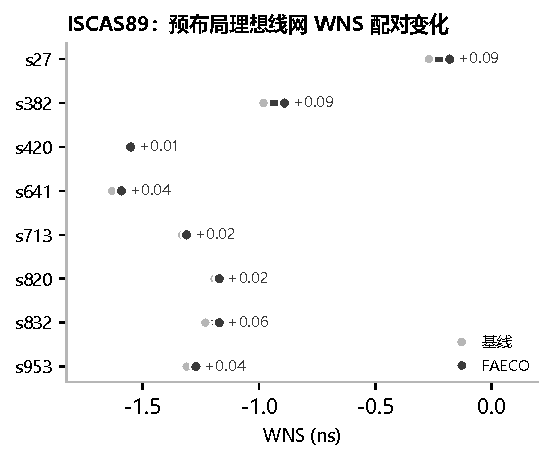
\includegraphics[width=1.0\columnwidth]{data/final/r27_monochrome/fig_iscas89/fig_iscas89.pdf}
\caption{ISCAS89 顺序电路混合修复的基线与 FAECO 结果对比（周期 0.5 ns；标注为 FAECO 相对基线的 WNS 变化）}
\label{fig:iscas_main}
\end{figure}

\begin{table}[htbp]
\centering
\caption{效率优先修复网表对的顺序等价证明}
\label{tab:sec_iscas8}
\setlength{\tabcolsep}{4pt}
\footnotesize
\begin{tabular}{lrrr}
\toprule
\textbf{电路} & \textbf{已证明/未证明} & \textbf{SEC} & \textbf{耗时 (s)} \\
\midrule
s27 & 11/0 & 通过 & 0.281 \\
s382 & 90/0 & 通过 & 0.281 \\
s420 & 79/0 & 通过 & 0.250 \\
s641 & 124/0 & 通过 & 0.313 \\
s713 & 126/0 & 通过 & 0.328 \\
s820 & 139/0 & 通过 & 0.344 \\
s832 & 146/0 & 通过 & 0.391 \\
s953 & 228/0 & 通过 & 0.407 \\
\bottomrule
\multicolumn{4}{p{0.92\columnwidth}}{\footnotesize 八对网表在同一批次使用Yosys0.33和共同SKY130行为模型，依次执行\texttt{proc/memory}、\texttt{equiv\_make}、\texttt{flatten}、\texttt{equiv\_simple}、\texttt{equiv\_induct -seq 10}及\texttt{equiv\_status -assert}。按本表行序，simple新增证明点为2/2/2/1/1/1/1/2，其余已由结构归并等建立；进入induct时八例均无未证明点，故归纳新增均为0。对应DFF数量为3/21/16/19/19/5/5/29，逐实例CK/D/Q映射相同。证明不依赖“先相等10周期”的额外同步假设；耗时仅为独立证明墙钟时间。}\\
\end{tabular}
\end{table}

\subsection{跨测试集评估}\label{sec:ood}

\subsubsection{ITC-99 基准族}\label{sec:itc99}

在纳入统一批量评估的 19 个 ITC-99 电路中，18 个电路的 WNS 取得严格改善，b06 与基线持平（$\Delta = 0\,\text{ns}$），19 个电路均无 WNS 回退。b17 在默认 60\,s 单候选验证时限下所有候选均触发 F5 超时而被拒，将其单候选验证时限放宽至 180\,s（其余 18 个电路仍用默认）后，在 104 条候选评估记录内取得 $+0.38\,$ns 改善（接受 G 候选 nor4b$_1\!\to\!$nor4b$_2$）。纳入统计的大规模电路 b14/b15/b17/b20/b21/b22 均取得严格 WNS 改善。b06 的基线 WNS 为 $-0.56\,\text{ns}$，其关键路径包含多个相邻的 \texttt{or4b$_1$} 单元。当前 R/G/B/JOINT 搜索中，G 类替换受到输入电容变化的限制，而 B/R 策略未能形成有效改善；664 条候选评估记录后，未观察到严格 WNS 改善。

接受候选以 G 为主：19 个电路中 17 个含 G 类接受（累计 69 次），B 与 R 类接受分别出现于 14 个和 10 个电路；收益最大的 b20/b21（分别为 $+1.98$ 和 $+2.75\,\text{ns}$）均以 G 为主、辅以 R。19 个电路共记录 3363 条候选评估，其中 2994 条 STA 结果具有可逐项核对的独立候选报告来源。19 个电路改善量的中位数为 $+0.18\,\text{ns}$、均值为 $+0.43\,\text{ns}$，两者的差异主要来自 b20 和 b21 较大的 WNS 改善幅度（其基线 WNS $\le -13\,\text{ns}$）。各失效类型在 19 个电路上的触发次数见表~\ref{tab:f16_dist}。表~\ref{tab:f16_dist} 的 F1--F6 触发分布表明，失败候选给出了可用的搜索诊断信息。

本节的候选评估次数按逐候选台账记录统计，包含前置拒绝与缓存复用，不直接等同于新执行的 STA 次数。

作为大规模补充实例（未纳入上述 19 个电路的统一统计）：b18（SKY130 映射后 7.57 万个单元）的 WNS 在 0.5 ns 下由 $-13.34$ ns 改善至 $-13.27$ ns，经 24 次候选级 STA 测量完成修复；b19（15.10 万个单元）由 $-17.44$ ns 改善至 $-16.00$ ns，经 59 次完成。

\subsubsection{PicoRV32 异构族}

基于同一寄存器传输级（RTL）源的三个结构差异明显的子模块直接复用 ISCAS89 流程。其中 PicoRV32 主核与其 PCPI 乘法协处理器 \texttt{picorv32\_pcpi\_mul} 具有有效 setup 路径，分别获得 $+1.13$ 和 $+0.07\,$ns 的改善（修复网表由 R/G/B 多类接受补丁叠加形成）；存储密集子模块 \texttt{picorv32\_regs} 为存储簇、无可建立 setup 路径，因此未执行时序修复，不参与改善判定。

\subsubsection{跨测试集功能验证}\label{sec:crossset_validation}

统一跨测试集评估的WNS严格改善比例分别为8/8、18/19和2/2。ITC-99的b17端点与原始接受记录、候选全文及新证明输入一致：仅实例\texttt{\_184320\_}由nor4b\_1变为nor4b\_2，WNS从$-16.53$到$-16.15$\,ns；完整单元模型、层次展开及断言检查得到12879个已证明点、0个未证明点，独立证明耗时13.375\,s。该计数来自这一明确网表对的新证明，不替换旧日志中的12812加1个未证明点记录。

模型审计还发现b09、b20和b21使用真实三态单元，其归档二态模型遗漏输出使能语义，故这三例只能保留时序测量，不能据二态SEC宣称功能已验证。16个支持域实例中15个严格改善，平均/中位改善为0.208/0.18\,ns；三态组的三个时序观察平均改善1.61\,ns。两组分层报告，避免将较大的未验证收益并入已验证功能子集。其余保留模型未发现实际使用单元的函数缺陷，但运行时模型内容摘要未全部归档，不据保留文件补造旧运行身份。恢复三态组功能证据需要保持真实输出使能与Z语义的证明流程，并对同一原始端点重新验证。

PicoRV32主核与乘法器另以完整行为模型进行独立证明，并核对两侧孤立常量X来源的结构身份；该分离证据不扩大为一般四态SEC。无setup路径的\texttt{picorv32\_regs}保持基线输出，不参与改善和证明分母。

三个测试集中各实例的 WNS 改善量见图~\ref{fig:unified_gain}。图中统一采用跨测试集迭代配置，保留 b06 的零改善及无 setup 路径子模块的非适用状态。

\begin{figure*}[!tb]
\centering
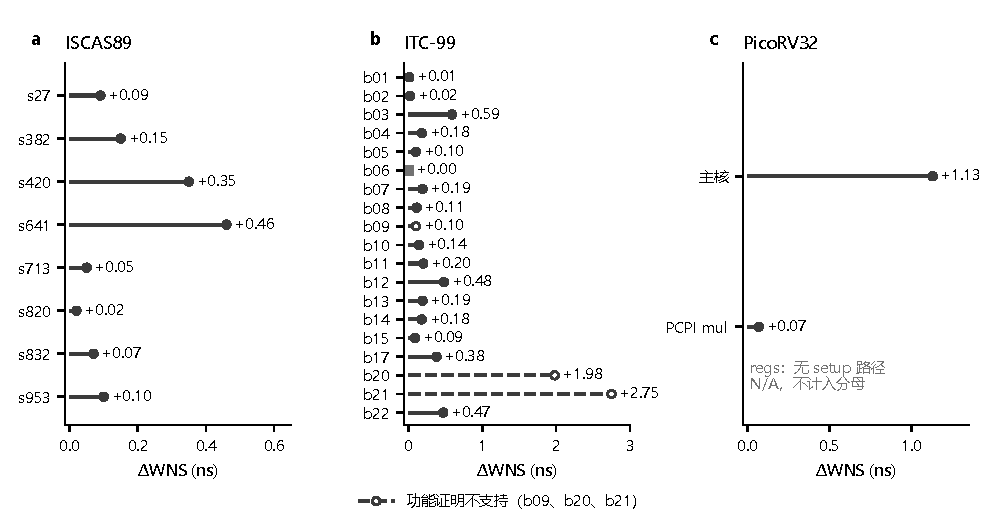
\includegraphics[width=0.92\textwidth]{data/final/r27_monochrome/r24_unified_status/fig4_r24.pdf}
\caption{统一迭代配置的逐实例预布局 WNS 改善。三个面板分别展示 ISCAS89、ITC-99 和 PicoRV32 的全部可评估实例，各面板横轴量程不同。改善量以各电路的基线为参照；b17 使用 180\,s 单候选时限，其余默认 60\,s。PicoRV32 主核、乘法器与 regs 的周期分别为 5、2 和 0.5\,ns；regs 无 setup 路径，不计入改善分母。空心端点和虚线标记b09、b20、b21的真实三态超出归档二态证明模型支持域；时序观察保留，不计为功能证明通过。图为归档单次运行的描述性结果。}
\label{fig:unified_gain}
\end{figure*}

\section{独立实验族、策略与反馈配置}
\begin{table*}[!t]
\centering
\caption{实验问题与配置对应关系}\label{tab:experiment_map}
\footnotesize\setlength{\tabcolsep}{4pt}
\begin{tabular}{>{\raggedright\arraybackslash}p{2.0cm}>{\raggedright\arraybackslash}p{4.8cm}>{\raggedright\arraybackslash}p{8.4cm}}
\toprule
\textbf{实验组} & \textbf{回答的问题} & \textbf{配置与结果用途} \\
\midrule
割边界受控对照 & 覆盖区域、节点代价与区域顺序分别有何作用 & 固定快照、输入与接受谓词；20轮/20提交、500新候选STA预约上限、8区域/轮、8实例/区域、单worker；关闭反馈、proxy、结构重综合和物理门控；见主文第4节 \\
单轮修复 & 首个改善候选及其后验质量 & 单轮首改进停止；独立证明与物理后验绑定同一对网表，见\S\ref{sec:iscas}、\S\ref{sec:phys_closure} \\
统一跨测试集 & 多种结构上取得的时序结果 & 最多8轮、可选反馈，b06保留TNS辅助接受、b17验证时限180s；按模型支持域分层，见\S\ref{sec:ood} \\
策略枚举 & 扩展修改类型的组合效果 & 最多20轮，混合臂含JOINT/TNS辅助、随机臂为RGB；未使用本节定义的两类边界，见\S\ref{sec:ablation} \\
排序反馈 & 固定与EMA的终点及开销 & 保留各自运行器及实际STA台账；不并入割机制归因，见\S\ref{sec:ablation} \\
结构扩展 & 深度下降能否转化为时序收益 & 独立窗口、重综合与映射流程，见\S\ref{sec:s_boundary} \\
\bottomrule
\end{tabular}
\end{table*}
\begin{table}[!htb]
\centering
\caption{效率优先与 20 轮迭代配置的关键参数对比}
\label{tab:configs}
\scriptsize
\setlength{\tabcolsep}{4pt}
\begin{tabular}{lcc}
\toprule
\textbf{参数} & \textbf{效率优先} & \textbf{20 轮迭代} \\
\midrule
最大迭代轮数                    & 1（首改进即停止） & 20 \\
F1--F6 失效反馈                  & 启用 & 不启用（固定权重） \\
10\,ps 物理门控 SPEF 复测        & 关 & 关 \\
单候选验证时限（默认）           & 60\,s & 60\,s \\
\bottomrule
\multicolumn{3}{p{0.95\columnwidth}}{\footnotesize 注：20 轮迭代配置（\S\ref{sec:ablation}）各列由固定权重运行器产生，用于比较候选空间与候选排序；跨测试集实验（\S\ref{sec:ood}）最多迭代 8 轮、启用跨轮失效反馈，其余关键参数与效率优先配置相同；效率优先配置虽启用失效反馈，但受单轮上限约束，权重更新不作用于任何候选构造，故其结果与固定权重一致；b17 的验证时限例外（180\,s）属跨测试集实验（\S\ref{sec:itc99}）。}\\
\end{tabular}
\end{table}
\subsection{候选空间、排序与反馈消融}\label{sec:ablation}

本节分两组实验。第一组采用历史关键实例策略枚举运行器，在 20 轮上限下比较局部修改策略配置（表~\ref{tab:ablation}），并记录首次取得改善所需的候选级 STA 次数（表~\ref{tab:efficiency}）。该运行器按关键实例枚举候选并在轮内逐实例提交，未使用式~\eqref{eq:cost} 的加权割与覆盖割；混合配置启用 TNS 辅助接受。混合配置包含 R/G/B/JOINT，随机配置仅枚举 R/G/B，因此两者的差异反映候选构造与评估顺序的联合作用。

固定搜索权重下，混合策略在 8 个 ISCAS89 电路上的平均 WNS 改善为 1.07\,ns，高于纯 G 的 0.16\,ns 和纯 B 的 0.54\,ns；随机策略三种子的平均改善为 0.40\,ns。各列共享 20 轮上限，实际候选级 STA 消耗不同。首次取得改善所需的 STA 次数在 7 个有台账的电路中，有 6 个混合策略少于随机策略三种子均值，s713 则相反；同一电路的不同随机种子间最大相差 7 倍。该对照刻画策略配置的搜索效果与启动开销，该组未隔离两类割，不能用于割机制归因；对应受控检验见主文第4节。

第二组检验失效反馈的独立作用：保持候选空间、初始权重与运行器的 STA 预约上限（500）不变，两配置均采用 20 轮迭代上限并启用提前停止，分别使用固定权重（Fixed）与 EMA 自适应更新（Adaptive）。定义 $B(k)$ 为截至第 $k$ 次新 STA 测量的累计最优 WNS 改善（best-so-far 曲线），两种配置在 8 个 ISCAS89 电路上的最终 $\Delta\mathrm{WNS}$、首次改善位置和最大 $B(k)$ 均相同，未观察到 EMA 反馈带来的额外收益。因此，本文将 F1--F6 用于失效分类与搜索分析。在第二组的两类配置下，取得相同终点所需的搜索开销见表~\ref{tab:runtime}；表中另列随机排序作为对照。

图~\ref{fig:budget_curves} 展示第二组实验的 $B(k)$ 曲线，按各臂新 STA 测量次数比较收益积累。固定权重与 EMA 自适应的收益积累相近，搜索终止位置不同；随机策略在不同电路与种子间表现不同，其中 s953 的三个随机种子终点均高于固定权重配置。曲线保留各臂的实际停止位置，以区分终点收益与到达该收益的测量开销。

\begin{figure*}[!tb]
\centering
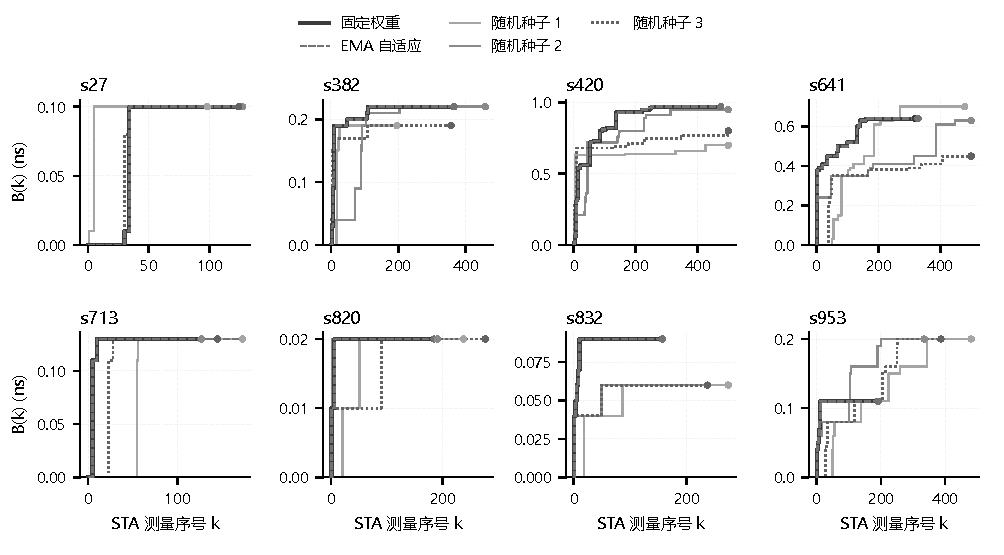
\includegraphics[width=0.92\textwidth]{data/final/r27_monochrome/fig5_budget_curves_r21/fig5_budget_curves_r21.pdf}
\caption{同一运行器配置下的收益积累曲线。横轴 $k$ 为从逐候选台账重建的新 STA 测量次数，保留具有 STA 来源且非缓存复用的记录，排除前置拒绝与缓存命中，纵轴为相对基线的累计最优 WNS 改善；圆点表示该臂实际停止位置，曲线不延伸至停止之后。全部 8 个电路与 3 个随机种子均展示，未作跨电路平均或插值。各臂逐电路的 STA 预约上限为 500；基线测量与最终 SEC 不计入横轴。该反馈对照族与表~\ref{tab:ablation} 的历史策略枚举对照分开统计。}
\label{fig:budget_curves}
\end{figure*}

\begin{table}[H]
\centering
\caption{ISCAS89 局部修改策略配置的 WNS 改善对比（周期 0.5\,ns）}
\label{tab:ablation}
\scriptsize
\setlength{\tabcolsep}{3pt}
\begin{tabular}{lrrrr}
\toprule
\textbf{电路} & \textbf{纯 G} & \textbf{纯 B} & \textbf{随机} & \textbf{混合 20 轮} \\
\midrule
s27  & +0.09 & +0.28 & +0.28 & \textbf{+0.28} \\
s382 & +0.17 & +0.19 & +0.19 & \textbf{+1.00} \\
s420 & +0.35 & +1.00 & +1.15 & \textbf{+1.54} \\
s641 & +0.45 & +1.27 & +0.57 & \textbf{+1.63} \\
s713 & +0.05 & +0.99 & +0.64 & \textbf{+1.33} \\
s820 & +0.02 & +0.26 & +0.15 & \textbf{+0.99} \\
s832 & +0.07 & +0.06 & +0.08 & \textbf{+0.57} \\
s953 & +0.09 & +0.24 & +0.12 & \textbf{+1.25} \\
\midrule
\textbf{均值} & 0.16 & 0.54 & 0.40 & \textbf{1.07} \\
\bottomrule
\multicolumn{5}{p{0.92\columnwidth}}{\footnotesize 数字为 WNS 改善量 (ns)，正值代表修复后 WNS 较基线提高。纯 G / 纯 B 列为单策略配置；随机列包含 R/G/B，随机化实例内候选顺序并取种子 1、2、3 的均值；混合列另含 JOINT。四列均不启用 F1--F6 权重重整，采用同一 20 轮上限，实际 STA 消耗不同；混合配置保留 WNS 持平时的 TNS 辅助接受。各臂完整命令未全部归档，本表报告历史策略配置的结果。} \\
\end{tabular}
\end{table}

\begin{table}[!htb]
\centering
\caption{首次取得改善所需的候选级 STA 次数（8 个 ISCAS89 电路，周期 0.5\,ns）}
\label{tab:efficiency}
\scriptsize
\setlength{\tabcolsep}{2pt}
\begin{tabular}{lccccc}
\toprule
\textbf{电路} & \textbf{混合策略} & \multicolumn{3}{c}{\textbf{随机策略}} & \textbf{随机均值} \\
\cmidrule(lr){3-5}
 & & \textbf{种子 1} & \textbf{种子 2} & \textbf{种子 3} & \\
\midrule
s27  & 1 & 3 & 3 & 1 & 2.3 \\
s382 & --- & 6 & 3 & 8 & 5.7 \\
s420 & 2 & 5 & 1 & 1 & 2.3 \\
s641 & 1 & 7 & 5 & 1 & 4.3 \\
s713 & 7 & 1 & 5 & 2 & 2.7 \\
s820 & 1 & 1 & 3 & 1 & 1.7 \\
s832 & 1 & 1 & 2 & 1 & 1.3 \\
s953 & 1 & 3 & 1 & 1 & 1.7 \\
\bottomrule
\multicolumn{6}{p{0.95\columnwidth}}{\footnotesize 数字为整次运行中第一个严格优于基线的候选所处的累积候选序号，即首次取得改善时已消耗的候选级 STA 次数；随机策略列为随机化实例内候选顺序的三个种子，随机均值为三者的算术平均。混合策略在 7 个有台账的电路中有 6 个少于随机均值（s713 相反），不同种子间最大相差 7 倍。s382 的混合策略逐候选台账缺失，该格留空。本表与表~\ref{tab:ablation} 同属历史 20 轮策略枚举配置；混合与随机策略的候选类型集合不同。} \\
\end{tabular}
\end{table}

\begin{table}[!htb]
\centering
\caption{20 轮迭代配置下的候选评估计数与搜索运行时间（8 个 ISCAS89 电路）}
\label{tab:runtime}
\footnotesize
\setlength{\tabcolsep}{2pt}
\begin{tabular}{>{\raggedright\arraybackslash}p{2.45cm}rrr}
\toprule
\textbf{配置} & \textbf{新 STA} & \textbf{评估记录} & \textbf{时间 (s)} \\
\midrule
固定权重（候选排序） & 1947 & 4146 & 2010.8 \\
EMA 自适应 & 2003 & 4883 & 2065.3 \\
随机排序（三种子均值） & 2480.7 & 5624 & 2460.3 \\
\bottomrule
\multicolumn{4}{p{0.95\columnwidth}}{\footnotesize 各臂采用 20 轮上限、提前停止与逐电路 STA 预约上限 500。新 STA 为具有 STA 来源且未标记缓存复用的候选记录数；评估记录包含前置拒绝与缓存复用。前两行为 8 电路合计，随机行为三个种子的各电路合计均值；其新 STA 合计分别为 2439、2476、2527。时间含候选构造、映射与候选级 STA，不计最终 SEC。本表与表~\ref{tab:ablation}、表~\ref{tab:efficiency} 的历史运行配置不同。}\\
\end{tabular}
\end{table}


\begin{table}[!htb]
\centering
\caption{F1--F6 失效触发次数（ITC-99 主实验）}
\label{tab:f16_dist}
\scriptsize
\setlength{\tabcolsep}{3pt}
\begin{tabular}{lcccccc}
\toprule
 & \textbf{F1} & \textbf{F2} & \textbf{F3} & \textbf{F4} & \textbf{F5} & \textbf{F6} \\
\midrule
触发次数 & 138 & 3 & 16 & 2434 & 915 & 0 \\
\bottomrule
\multicolumn{7}{p{0.95\columnwidth}}{\footnotesize 统计范围为 19 个 ITC-99 电路、4044 次候选级评估。F4 对应未满足接受判据的候选，占候选级评估的 60.2\%，是本配置下的主导失效类型；F6 只在启用物理门控时触发，本配置未启用，故为 0。本表保留 b17 默认 60\,s 批次的 785 次评估；跨测试集结果及 3363 条评估记录采用其 180\,s 重跑的 104 次评估。} \\
\end{tabular}
\end{table}

\section{网表代价与物理后验}
\begin{table}[htbp]
\centering\caption{W1端点的网表代价}\label{tab:netlist_cost}
\footnotesize\setlength{\tabcolsep}{3pt}
\begin{tabular}{lrrr}
\toprule
\textbf{电路} & \textbf{单元数前/后} & \textbf{缓冲前/后} & \textbf{库面积变化(\%)}\\
\midrule
s27 & 11/11 & 0/0 & 4.76 \\
s382 & 90/90 & 0/0 & 1.55 \\
s420 & 79/79 & 0/0 & 4.92 \\
s641 & 122/122 & 0/0 & 2.07 \\
s713 & 124/124 & 0/0 & 0.27 \\
s820 & 138/138 & 0/0 & 0.29 \\
s832 & 145/145 & 0/0 & 0.71 \\
s953 & 228/228 & 0/0 & 0.80 \\
\bottomrule
\multicolumn{4}{p{0.93\columnwidth}}{\footnotesize 单元数包含逐实例展开的DFF，缓冲数统计独立buf/clkbuf单元；面积为同一Liberty库的单元面积属性之和的相对变化，不是布局核心面积或功耗估计。各行与W1的初始/最终原始网表摘要绑定。}\\
\end{tabular}
\end{table}
\subsection{预布局候选筛选的物理相关性分析}\label{sec:phys_closure}

本实验考察\S\ref{sec:eff_prio}单轮候选在布局和全局布线寄生估计下的收益保持情况，独立于割边界受控配置。图~\ref{fig:physical_transfer}和表~\ref{tab:pr8}保留全部8例：5个改善、1个持平、2个退化，退化分别为0.02和0.01\,ns。需要说明，这是单一物理实现点上的读数：同族同网表对在其它已归档实现上出现符号翻转，而各例差值均落在实现轴的变化范围内，故只记为实现轴敏感的观察，不据此断言改善方向在物理估计下是否保持。每例基线与候选使用字节相同的OpenROAD脚本，TT25℃、1.8\,V、CK周期0.5\,ns；s27利用率10\%，其余30\%，布局密度0.7。时序寄生由\texttt{estimate\_parasitics -global\_routing}给出，不称为最终签核结果。脚本未显式设置I/O延迟、外加输出负载、输入转换时间及额外时钟不确定度，运行时平台全文件及随机种子身份也未完整保留；这些条件限定了物理结果的可复验范围。


\begin{figure}[!htb]
\centering
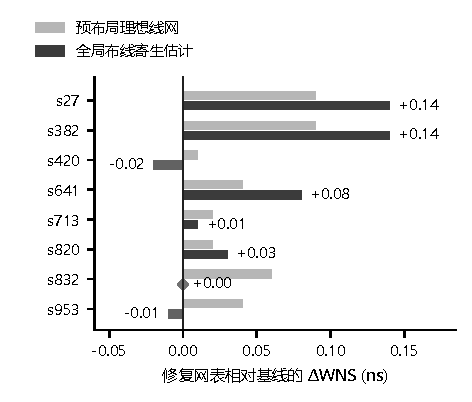
\includegraphics[width=0.92\columnwidth]{data/final/r27_monochrome/fig6_physical_transfer_r21/fig6_physical_transfer_r21.pdf}
\caption{效率优先候选的收益保持情况。每组柱对应同一电路、同一接受候选，分别以预布局理想线网与全局布线寄生估计条件下的基线为参照。八电路全部纳入（单一物理实现点），物理估计后 5 个改善、1 个持平、2 个退化；负值柱表示退化，菱形表示持平。该单轮候选族与图~\ref{fig:unified_gain} 的迭代主结果分开统计。}
\label{fig:physical_transfer}
\end{figure}

简化线载试验与OpenROAD几何寄生估计分开。对网$e$，估计器采用
\begin{equation}\label{eq:estimated_rc}
\begin{aligned}
L(e)&=\ell\max\{1,\sqrt{F(e)}\}\,p_f p_d,\\
R(e)&=0.09\,L(e)\ [\Omega],\\
C(e)&=0.00021\,L(e)\ [\mathrm{pF}],
\end{aligned}
\end{equation}
其中$\ell$以$\mu$m计，$F(e)$为生成器记录的扇出数，$p_f,p_d$均为全局乘数，设为1；它不从坐标或曼哈顿距离提取线长，$p_d$也不是逐网深度。单位电阻0.09\,$\Omega/\mu$m、单位电容0.21\,fF/$\mu$m作为敏感性模型的设定，不宣称经过物理提取标定；该RC为估算值，非签核级提取。寄生文件仅含估计线电容，引脚电容仍由Liberty提供；线电容集中到驱动端，电阻按星形支路分配。

归档线载扫描曾对基线与候选共用基线SPEF，s382候选还出现缺引脚告警，因此不能据其曲线认定收益衰减或门控有效。门控记录中的s382与b18分别有50条和6条评估，但仅对应5个和1个不同候选全文；b18保留SPEF与1\,$\mu$m单位长度匹配，s382的原始RC配方未恢复，不能将它们统一记作40\,$\mu$m、56个独有候选。本文保留这些记录用于来源与计数审计，不用其估计物理失败率。有效的双侧后验须由各自网表生成寄生文件，核对所有层级引脚的实际注入；仅返回码为0或同网表时序差值为0不足以通过这项验收。

为检验负载敏感性，另对C′覆盖优先臂的s382初末网表实施配对后验。原层级网表的首个同网表控制出现43组部分未注释驱动，故停止而不采其时序值。后续仅展开用户DFF辅助层级，逐端口、单元与引脚核对90个标准单元和21个寄存器的连接，未重新综合或改变单元；原初始和最终网表到各自展开网表的独立二态SEC均为129/0。这个派生输入族与原层级输入分开登记。

在展开后的同一初始网表上，$\ell=40\,\mu$m双侧控制的理想线网及SPEF时序差均为0；两个SPEF字节相同，两侧真实注释报告均无未注释或部分未注释驱动。随后以各自网表生成寄生，在$\ell=10,40,160\,\mu$m下重新测量同一候选对，结果见主文表6。全部8次注释回放均无注释缺口，并与对应STA结果一致。理想线网改善0.15\,ns，在最小基础长度下保留0.11\,ns，较大两点的改善均降至0.01\,ns的报告粒度以下，记为零读数而非已证实的效应消失。因此，即使单元功能与连接保持，理想线网增益也可能随简化线载消失；本试验不把该设定下的长度解释为实际布线长度。

主文表6给出该派生端点对的三点测量结果；每点都重新测量理想线网时序，16次测量与8次注释回放共24次STA，与最初失败的5次分开。



\begin{table}[ht]
\centering
\caption{OpenROAD 布局及全局布线寄生估计后的 WNS 对比（8 个 ISCAS89 电路）}
\label{tab:pr8}
\footnotesize
\setlength{\tabcolsep}{2pt}
\begin{tabular}{lrrrrr}
\toprule
 & \multicolumn{2}{c}{\textbf{预布局}} & \multicolumn{2}{c}{\textbf{全局布线估计}} & \\
\cmidrule(lr){2-3}\cmidrule(lr){4-5}
\textbf{电路} & \textbf{基线} & \textbf{修复} & \textbf{基线} & \textbf{修复} & $\Delta$ \\
\midrule
s27  & $-0.27$ & $-0.18$ & $-0.36$ & $-0.22$ & $+0.14$ \\
s382 & $-0.98$ & $-0.89$ & $-1.16$ & $-1.02$ & $+0.14$ \\
s420 & $-1.56$ & $-1.55$ & $-1.80$ & $-1.82$ & $-0.02$ \\
s641 & $-1.63$ & $-1.59$ & $-2.10$ & $-2.02$ & $+0.08$ \\
s713 & $-1.33$ & $-1.31$ & $-1.59$ & $-1.58$ & $+0.01$ \\
s820 & $-1.19$ & $-1.17$ & $-1.52$ & $-1.49$ & $+0.03$ \\
s832 & $-1.23$ & $-1.17$ & $-1.51$ & $-1.51$ & $0.00$ \\
s953 & $-1.31$ & $-1.27$ & $-1.60$ & $-1.61$ & $-0.01$ \\
\bottomrule
\multicolumn{6}{p{0.92\columnwidth}}{\footnotesize 各例均为对应单轮基线及其接受候选；s27利用率10\%，其余30\%，两侧相同脚本，TT25℃/1.8V/0.5ns；$\Delta$ 为全局布线寄生估计后修复网表相对基线的 WNS 变化。}\\
\end{tabular}
\end{table}

\section{结构候选的负结果}
\subsection{结构候选扩展与能力边界}\label{sec:s_boundary}

除 R/G/B/JOINT 构造级变换外，本文还实现了一类窗口局部结构重综合候选（记为 S），用于评估其是否带来额外的 WNS 改善。为考察候选数量的影响，本文扩大 S 的候选池并做开关对照：关闭 S 后，8 个电路的结果均与原配置一致，两臂的非 S 候选序列一致，候选级 STA 预算未触及上限。结构候选（S）的能力边界见表~\ref{tab:s_boundary}。

候选级深度变化与 WNS 变化的逐电路分布见图~\ref{fig:s_candidate_outcomes}，两类指标分别统计，避免将逻辑深度下降解释为时序收益。

\begin{figure}[!htb]
\centering
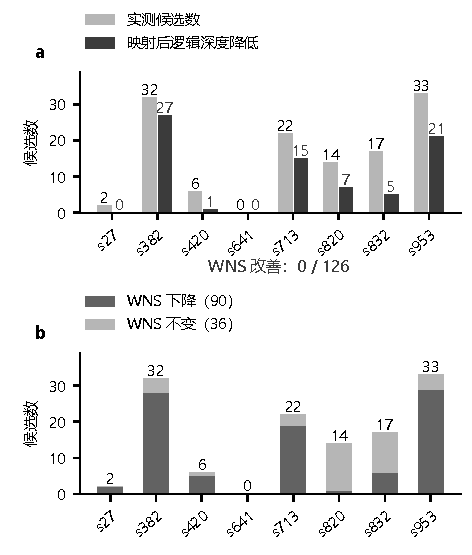
\includegraphics[width=0.92\columnwidth]{data/final/r27_monochrome/fig7_s_boundary_r21/fig7_s_boundary_r21.pdf}
\caption{扩大候选池后的 S 候选结果。上图比较候选数与 SKY130 映射后逻辑深度降低的候选数；下图按 WNS 不变或下降分类，两图为同一批 126 个候选的不同分类维度。8 个电路全部展示，其中 s641 未成功抽取窗口，候选数为零。76 个候选降低深度，WNS 改善为 0/126；同预算 S 开关对照的 8 个电路终点 WNS 均不变。}
\label{fig:s_candidate_outcomes}
\end{figure}

\begin{table}[H]
\centering
\caption{结构候选（S）的能力边界}
\label{tab:s_boundary}
\footnotesize
\setlength{\tabcolsep}{8pt}
\begin{tabular}{lrr}
\toprule
\textbf{指标} & \textbf{原配置} & \textbf{扩大候选池} \\
\midrule
S 候选数 & 37 & 126 \\
$\Delta L>0$ & — & 76/126 \\
$\Delta_{\mathrm{WNS}}>0$ & 0 & 0/126 \\
$\Delta_{\mathrm{WNS}}=0$ & — & 36/126 \\
$\Delta_{\mathrm{WNS}}<0$ & — & 90/126 \\
接受电路 & 0/8 & 0/8 \\
\bottomrule
\multicolumn{3}{p{0.9\columnwidth}}{\footnotesize $\Delta L=L_{\mathrm{before}}-L_{\mathrm{after}}$，正值表示 SKY130 映射后逻辑深度降低；$\Delta_{\mathrm{WNS}}=\mathrm{WNS}_{\mathrm{after}}-\mathrm{WNS}_{\mathrm{before}}$，正值表示时序改善。$\Delta L$ 与 $\Delta_{\mathrm{WNS}}$ 为两个相互独立的分类维度，同一候选可同时计入两类，故各行数量不要求相加等于候选总数。}\\
\end{tabular}
\end{table}



扩大候选池后，S 候选数量由 37 增至 126，其中 76 个候选降低了映射后的逻辑深度，但均未取得严格 WNS 改善，另有 90 个候选导致 WNS 下降（其余 36 个 WNS 不变）。结果表明，在当前窗口构造、重综合与映射流程下，扩大候选池并未带来额外 WNS 改善。因此，本文将 S 保留为可选候选类型，不将其计入主要性能贡献。

\section{数据与复核入口}

主文受控对照的运行器固定为\texttt{3ea0f75}，原输入、库摘要和72次验收见\nolinkurl{project_docs/evidence/r22_cprime_v3_20261016/MATRIX_AUDIT_72.json}。候选STA、提交曲线及W1网表代价分别见\nolinkurl{paper/zh/figures/data/final/r24_cp_gain_cost/}、\nolinkurl{paper/zh/figures/data/final/r24_cp_budget_curves/}和\nolinkurl{project_docs/evidence/r24_paper_revision_20261018/QUANTITATIVE_REUSE.json}。

主文线载后验生成器固定为\texttt{f761ee1}，保单元/状态展开输入、两份原到展开网表证明、原层级失败及新24次STA按对象分别归档于\nolinkurl{project_docs/evidence/r24_paper_revision_20261018/}。新结果不恢复原层级SPEF支持或旧共享SPEF扫描。

跨族归档结果尚有运行版本、模型与输入身份缺项；保留文件审核不补造旧运行身份。当前证据和未解决条目分别见\nolinkurl{project_docs/evidence/}与\nolinkurl{project_docs/OPEN_ISSUES.md}。

\end{document}
